\documentclass[10pt,a4paper]{beamer}
\usepackage[utf8x]{inputenc}
\usepackage{ucs}
\usepackage[english]{babel}
\usepackage{amsmath}
\usepackage{tikz}
\usetikzlibrary{shapes,arrows}
\usetikzlibrary{positioning, shapes}
\usetikzlibrary{trees,calc}
\usepackage{fancybox}
\usepackage{tikz-qtree}
\usepackage{amsfonts}
\usepackage{amssymb}
\author{Guillaume Maudoux \& Cédric Libert}
\title{Symbolic search}
\setbeamertemplate{navigation symbols}{%
}
\begin{document}
\maketitle
\begin{frame}
\tableofcontents
\end{frame}
\section{Intro}
\begin{frame}
\frametitle{The problem of storing many states}

The list of states still to explore in a classcial search can be very space-consuming (exponential in BFS).  One solution is to use DFS, but then memory usage is suboptimal.  We explore another structure able to store many states in a compressed way: the binary decision diagrams.

\end{frame}

\begin{frame}
\frametitle{Binary decision diagrams}

\begin{itemize}
\item BDDs encode a boolean function (def.)
\item BDDs seen as reduced decision trees
\end{itemize}

Boolean function example: $a\vee (\neg b \wedge \neg c) \rightarrow a$
%\tikzstyle{var} = [circle, draw, fill=blue!20,  align=center, minimum size = 1cm,
%     text badly centered, node distance=2cm, inner sep=2pt]
%\tikzstyle{line} = [draw, -latex']
%
%\begin{tikzpicture}
%\node[var] (a1) {a};
%\node[var,below left of=a1] (b1) {b};
%\node[var,below right of=a1] (b2) {b};
%\node[var,below left of=b1] (c1) {c};
%\node[var,below right of=b1] (c2) {c};
%\node[var,below left of=b2] (c3) {c};
%\node[var,below right of=b2] (c4) {c};
%
%\path [line] (a1) -- node [above] {1} (b1);	
%\path [line] (a1) -- node [above] {0} (b2);	
%
%\foreach \b/\c/\v in {b1/c1/1, b1/c2/0,b2/c3/1, b2/c4/0}
%    \path[line] (\b) -- node[above] {\v} (\c);
%
%\end{tikzpicture}

%\begin{tikzpicture}[ level 1/.style={sibling distance=3cm},
%  level 2/.style={sibling distance=1.5cm}]
%\node [circle,draw] (a){$a$}
%	child {node [circle,draw] (b1) {$b$}
%	    child {node [circle,draw] (c1) {$c$}
%	    		child {node {$1$} edge from parent node[above]{1}}
%	    		 child {node {$1$} edge from parent node[above]{0}}
%		}
%      	child {node [circle,draw] (c2) {$c$}
%      		      	}		     
%      	edge from parent node[above] {1}
%      }
%     child {node [circle,draw] (b2) {$b$}
%	    child {node [circle,draw] (c3) {$c$}
%	    		      	edge from parent node[above] {1}}
%      	child {node [circle,draw] (c4) {$c$}
%      				edge from parent node[above] {0}}
%      	edge from parent node[above] {0}		     
%     };
%\end{tikzpicture}
\tikzstyle{line} = [draw, -latex']

  \begin{overlayarea}{6cm}{1cm}
  	\only<1-2>{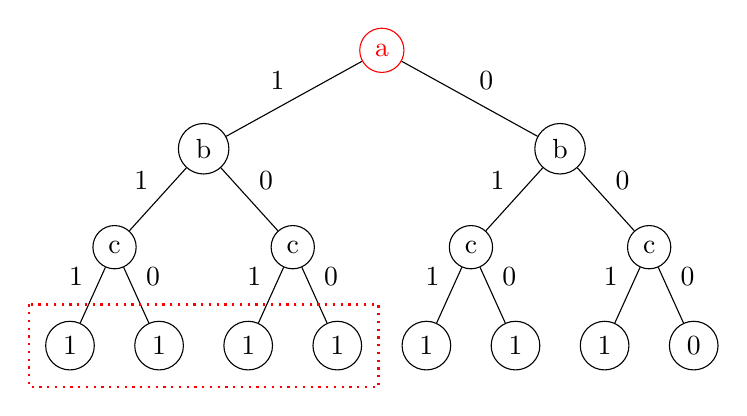
\begin{tikzpicture}
[every tree node/.style={draw,circle},
   level distance=1.25cm,sibling distance=.5cm, 
   edge from parent path={(\tikzparentnode) -- (\tikzchildnode)}]
\Tree [.\node[red](a) {a}; 
     \edge node[auto=right] {1};[.\node (b) {b};
        \edge node[auto=right] {1};[.c 
           \edge node[auto=right] {1}; [.\node (t1) {1}; ] \edge node[auto=left] {0}; [.\node (t2) {1}; ] 
        ]      
        \edge node[auto=left] {0};[.c 
          \edge node[auto=right] {1}; [.\node (t3) {1}; ] \edge node[auto=left] {0}; [.\node (t4) {1}; ] 
        ] 
    ]
      \edge node[auto=left] {0}; [.b
        \edge node[auto=right] {1}; [.c 
          \edge node[auto=right] {1}; [.1 ] \edge node[auto=left] {0}; [.1 ] 
        ] 
        \edge node[auto=left] {0}; [.c 
          \edge node[auto=right] {1}; [.1 ] \edge node[auto=left] {0}; [.0 ] 
        ]
    ] ]
    
        \onslide<2>{\draw[red,thick,dotted] ($(t1.north west)+(-0.3,0.3)$)  rectangle ($(t4.south east)+(0.3,-0.3)$);}
\end{tikzpicture}}
\only<3-4>{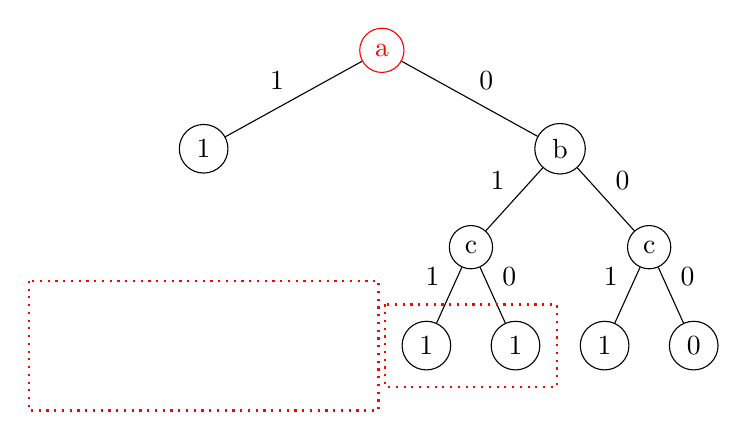
\begin{tikzpicture}
[every tree node/.style={draw,circle},
   level distance=1.25cm,sibling distance=.5cm, 
   edge from parent path={(\tikzparentnode) -- (\tikzchildnode)}]
\Tree [.\node[red](a) {a}; 
     \edge node[auto=right] {1};[.\node (b) {1};
        \edge[white];[.\node[white] (c) {c}; 
           \edge[white] node[auto=right] {1}; [.\node[white] (t1) {1}; ] \edge[white] node[auto=left] {0}; [.\node[white] (t2) {1}; ] 
        ]      
        \edge[white] node[auto=left] {0};[.\node[white] (c2) {c}; 
          \edge[white] node[auto=right] {1}; [.\node[white] (t3) {1}; ] \edge[white] node[auto=left] {0}; [.\node[white] (t4) {1}; ] 
        ] 
    ]
      \edge node[auto=left] {0}; [.b
        \edge node[auto=right] {1}; [.c 
          \edge node[auto=right] {1}; [.\node (t5) {1}; ] \edge node[auto=left] {0}; [.\node (t6) {1}; ] 
        ] 
        \edge node[auto=left] {0}; [.c 
          \edge node[auto=right] {1}; [.1 ] \edge node[auto=left]  {0}; [.0 ] 
        ]
    ] ]
    
        \onslide<2>{\draw[red,thick,dotted] ($(t1.north west)+(-0.3,0.6)$)  rectangle ($(t4.south east)+(0.3,-0.6)$);}
        \onslide<4>{\draw[red,thick,dotted] ($(t5.north west)+(-0.3,0.3)$)  rectangle ($(t6.south east)+(0.3,-0.3)$);}
\end{tikzpicture}}
\only<5-6>{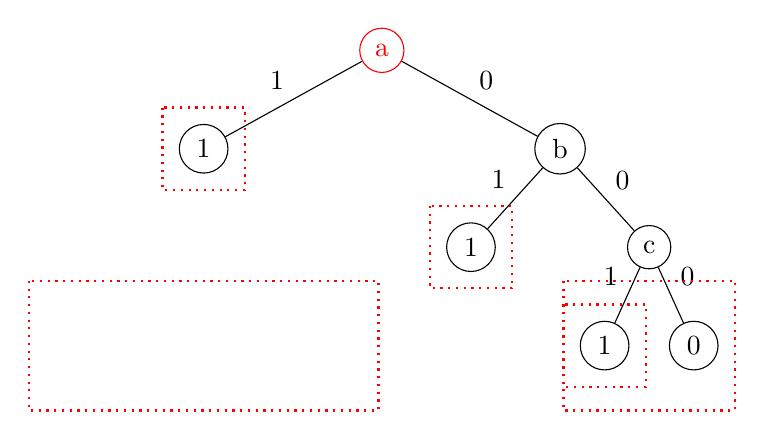
\begin{tikzpicture}
[every tree node/.style={draw,circle},
   level distance=1.25cm,sibling distance=.5cm, 
   edge from parent path={(\tikzparentnode) -- (\tikzchildnode)}]
\Tree [.\node[red](a) {a}; 
     \edge node[auto=right] {1};[.\node (b) {1};
        \edge[white];[.\node[white] (c) {c}; 
           \edge[white] node[auto=right] {1}; [.\node[white] (t1) {1}; ] \edge[white] node[auto=left] {0}; [.\node[white] (t2) {1}; ] 
        ]      
        \edge[white] node[auto=left] {0};[.\node[white] (c2) {c}; 
          \edge[white] node[auto=right] {1}; [.\node[white] (t3) {1}; ] \edge[white] node[auto=left] {0}; [.\node[white] (t4) {1}; ] 
        ] 
    ]
      \edge node[auto=left] {0}; [.\node (b2) {b};
        \edge node[auto=right] {1}; [.\node (c4) {1};
          \edge[white] node[auto=right] {1}; [.\node[white] (t5) {1};] \edge[white] node[auto=left] {0}; [.\node[white] (t6) {1}; ] 
        ] 
        \edge node[auto=left] {0}; [.\node (c5) {c}; 
          \edge node[auto=right] {1}; [.\node (t7) {1}; ] \edge node[auto=left]  {0}; [.\node (t8) {0}; ] 
        ]
    ] ]
    
        \onslide<2>{\draw[red,thick,dotted] ($(t1.north west)+(-0.3,0.6)$)  rectangle ($(t4.south east)+(0.3,-0.6)$);}
        \onslide<4>{\draw[red,thick,dotted] ($(t7.north west)+(-0.3,0.6)$)  rectangle ($(t8.south east)+(0.3,-0.6)$);}
        
        \onslide<6>{
        	\foreach \name in {b,c4,t7}
        	  \draw[red,thick,dotted] ($(\name.north west)+(-0.3,0.3)$)  rectangle ($(\name.south east)+(0.3,-0.3)$);}        
\end{tikzpicture}}
\only<7->{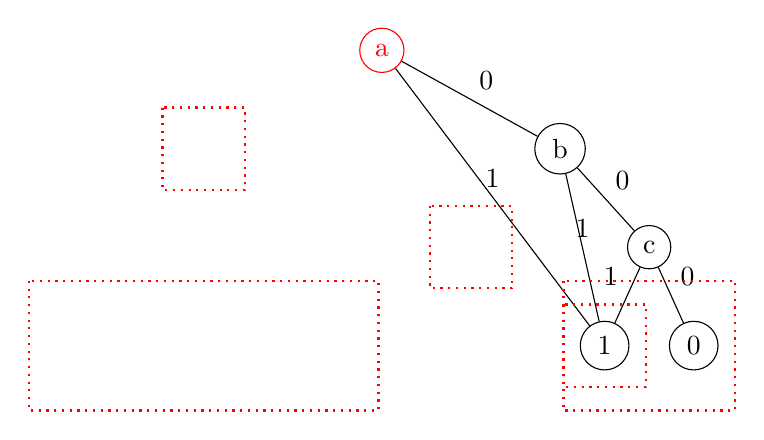
\begin{tikzpicture}
[every tree node/.style={draw,circle},
   level distance=1.25cm,sibling distance=.5cm, 
   edge from parent path={(\tikzparentnode) -- (\tikzchildnode)}]
\Tree [.\node[red](a) {a}; 
     \edge[white] node[auto=right] {1};[.\node[white] (b) {1};
        \edge[white];[.\node[white] (c) {c}; 
           \edge[white] node[auto=right] {1}; [.\node[white] (t1) {1}; ] \edge[white] node[auto=left] {0}; [.\node[white] (t2) {1}; ] 
        ]      
        \edge[white] node[auto=left] {0};[.\node[white] (c2) {c}; 
          \edge[white] node[auto=right] {1}; [.\node[white] (t3) {1}; ] \edge[white] node[auto=left] {0}; [.\node[white] (t4) {1}; ] 
        ] 
    ]
      \edge node[auto=left] {0}; [.\node (b2) {b};
        \edge[white] node[auto=right] {1}; [.\node[white] (c4) {1};
          \edge[white] node[auto=right] {1}; [.\node[white] (t5) {1};] \edge[white] node[auto=left] {0}; [.\node[white] (t6) {1}; ] 
        ] 
        \edge node[auto=left] {0}; [.\node (c5) {c}; 
          \edge node[auto=right] {1}; [.\node (t7) {1}; ] \edge node[auto=left]  {0}; [.\node (t8) {0}; ] 
        ]
    ] ]
    		\foreach \name in {a,b2}
    			\draw (\name) -- node[above] {1} (t7);
        \onslide<2>{\draw[red,thick,dotted] ($(t1.north west)+(-0.3,0.6)$)  rectangle ($(t4.south east)+(0.3,-0.6)$);}
        \onslide<4>{\draw[red,thick,dotted] ($(t7.north west)+(-0.3,0.6)$)  rectangle ($(t8.south east)+(0.3,-0.6)$);}
        
        \onslide<6>{
        	\foreach \name in {b,c4,t7}
        	  \draw[red,thick,dotted] ($(\name.north west)+(-0.3,0.3)$)  rectangle ($(\name.south east)+(0.3,-0.3)$);} 
    
\end{tikzpicture}}


  \end{overlayarea}


\end{frame}
\section{Representing  state sets with BDDs}
\begin{frame}
\frametitle{Representing  state sets with BDDs}
	\begin{itemize}
	\item BDDs use boolean vectors.  So we need a representation of states as boolean vectors.
	\item How do we represent a state ? A set of states ? A transition function ?
	\item Discussion about space efficency.
	\end{itemize}
\end{frame}

\section{Computing with BDDs}
\begin{frame}
\frametitle{Computing with BDDs}

\begin{itemize}
\item union
\item intersection
\item projection
\item quantification
\item time complexity of these operations
\end{itemize}

\end{frame}

\section{The BFS implemented with set operations}
\begin{frame}
\frametitle{The BFS implemented with set operations}
\end{frame}

\section{Adaptation of classical algorithms}
\begin{frame}
\frametitle{Adaptation of classical algorithms}

	\begin{itemize}
	\item Dijkstra
	\item A*: the additional difficulty due to usage of heuristics
	\end{itemize}
\end{frame}

\section{Fast pattern database with BBDs}
\begin{frame}
\frametitle{Fast pattern database with BBDs}

BDDs are an efficient way to implement pattern databases.
\begin{itemize}
\item What is a pattern database ?
\item How to implement it with BDDs ?
\item Is it really so efficient ?
\end{itemize}
\end{frame}

\section{Conclusion}
\begin{frame}
\frametitle{Conclusion}

\end{frame}

\end{document}